%%% -*- TeX-master: "case-study.tex" -*-
\section{The minmod limiter}
\label{sec:minmod}

Simulation of physical phenoma is an important use case for differential equation solvers, consequently ways to reduce or eliminate numerical errors have always been of interest.
One of the first ideas was researched by van Leer in 1979, when he proposed the $\minmod$ limiter\cite{VanLeer1979}.
A limiter in general restricts the steepness of the gradient of $U$ to sensible values where the bounds may be computed based on the current state or even set based on domain knowledge.
Of interest for us is in particular the former type because of its wide applicability.

The idea behind $\minmod$ specifically is to preserve the monotonicity of $U$.
% TODO: What is monotonicity? Does is provide TVD?
In the simplest case assume that the solution on cell $i$ is approximated by a first-order polynomial $c_{i}^{1}x + c_{i}^{0}$.
The limiter updates all the slopes $c_{i}^{1}$ to $\tilde{c}_{i}^{1}$ by
\begin{equation*}
  \tilde{c}_{i}^{1} = \minmod\left( c_{i}^{1}, \frac{c_{i + 1}^{0} - c_{i}^{0}}{\Delta x}, \frac{c_{i}^{0} - c_{i - 1}^{0}}{\Delta x} \right)
\end{equation*}
where the $\minmod$ operation is defined by
\begin{equation*}
  \minmod(a, b, c) = \begin{cases}
    \displaystyle\argmin_{x \in \{ a, b, c \}} |x| & \text{if} \sgn(a) = \sgn(b) = \sgn(c)\\
    0 & \text{otherwise}
  \end{cases}
\end{equation*}
So the slope on each cell is bounded by the forward and backward difference quotients of the cell and its neighbor's average values that approach the true first derivative as $\Delta x$ goes to $0$.
% TODO: How does this preserve monotonicity?

The effect of this limiter is demonstrated in figure \ref{fig:minmod}.
In figure \ref{fig:minmod-steep} the slope is limited so that the values do not exceed the average levels on neighboring cells.
Figure \ref{fig:minmod-extremum} shows how the approximation is reduced to first order in the case of an extremum as well as in the case that the slope does not agree with the trend set by the cell's neighbors (figure \ref{fig:minmod-trend}).
\begin{figure}[h]
  \centering
  \begin{subfigure}{0.5\columnwidth}
    \centering
    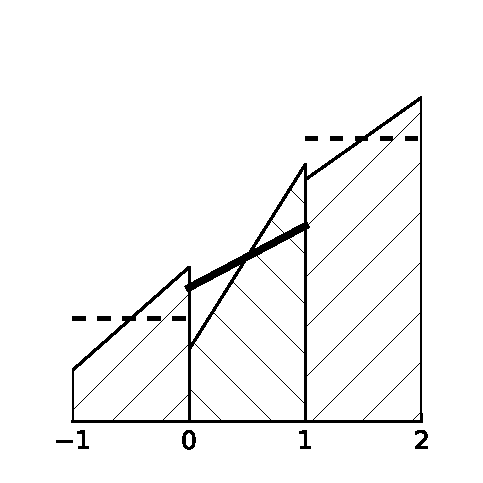
\includegraphics[width=\textwidth]{figures/minmod-a}
    \caption{Too steep}
    \label{fig:minmod-steep}
  \end{subfigure}
  \begin{subfigure}{0.5\columnwidth}
    \centering
    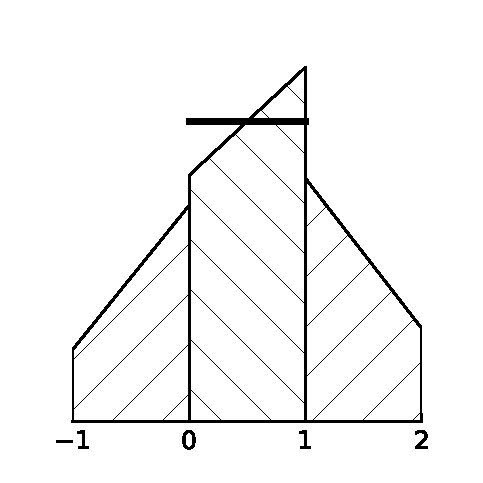
\includegraphics[width=\textwidth]{figures/minmod-b}
    \caption{Extremum in cell}
    \label{fig:minmod-extremum}
  \end{subfigure}
  \begin{subfigure}{0.5\columnwidth}
    \centering
    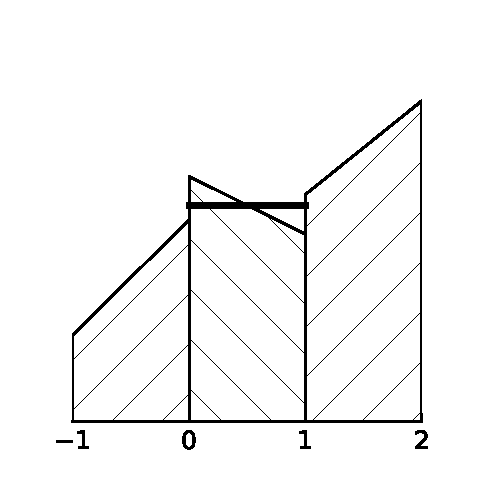
\includegraphics[width=\textwidth]{figures/minmod-c}
    \caption{Trend disagreement}
    \label{fig:minmod-trend}
  \end{subfigure}
  \caption{Three cell domain showcasing when the minmod limiter becomes active. Dashed line indicate average levels in a cell, bold lines designate limited slopes.}
  \label{fig:minmod}
\end{figure}

Prevent new extrema.
Generalization to higher orders.
reduces order to $1$.
